\chapter{Knowledge Graphs}
\label{cha:vkg}

\section{Cos'è un Knowledge Graph}
\label{sec:kg_description}

Si inizia a parlare di rappresentazione della conoscenza tramite l'aiuto di knowledge base già dalla fine degli anni 50 e nel 1980 ricercatori dell'università di Groningen 
e dell'università di Twente nei Paesi Bassi usarono per la prima volta il termine Knowledge Graph per descrivere il loro sistema basato sull'integrazione di molteplici sorgenti
di dati per rappresentare il linguaggio naturale tramite una knowledge base .
Questo primo momento di ricerca iniziale fu poi seguito all'inizio degli anni 2000 dall'affermazione degli standard W3C come RDF e OWL nell'ambito del 
Semantic Web a dal sorgere di varie ontologie pubbliche come DBPedia, YAGO e Freebase. \cite{KGDefinition} \cite{KGSurvey}

Il termine Knowledge Graph nasce però solo nel 2012 con il motore di ricerca di Google che introduce il termine per descrivere
le nuove funzionalità di ricerca semantica del proprio motore di ricerca: le ricerche che vengono effettuate non sono più semplice string matching,
ma viene aggiunta una componente di ragionamento di grado di riconoscere veri e propri "oggetti" del mondo reale. \cite{KGDefinition}

La definizione precisa di cosa sia un knowledge graph rimane nebulosa e definizioni differenti risultano essere a volte in contraddizione l'una con l'altra. 
In modo molto generale possiamo definire un knowledge graph come una struttura che rappresenta la conoscenza come un insieme di concetti e le relazioni fra essi.
Se vogliamo invece dare una definizione più formale possiamo definire un knowledge graph come una struttura che acquisisce e integra informazioni in una knowledge base
e applica un motore d'inferenza per ricavare nuova conoscenza come mostrato in figura \ref{fig:KG}.
Molte definizioni indicano anche la dimensione del KG come fattore determinante, ma cosa questo significhi nel dettaglio non è mia specificato.

La knowledge base è spesso implementata praticamente tramite ontologia e può quindi sfruttare tutte le caratteristiche che rendono i grafi un'ottima scelta per rappresentare 
conoscenza. In particolare i grafi risultano essere ottimi per modellare domini complessi in quanto gli archi possono rappresentare relazioni tra diversi nodi, che rappresentano 
i soggetti, anche molto complesse. Inoltre la mancanza di uno schema definito a priori permette all'insieme dei dati di crescere in modo più flessibile e i linguaggi di interrogazione
per sistemi basati su grafi sono molto espressivi e contengono la maggior parte dei costrutti usati da linguaggi di query più tradizionali come join, unioni, proiezioni, \dots \cite{KGIntro}.

\begin{figure}[h]
    \centering
    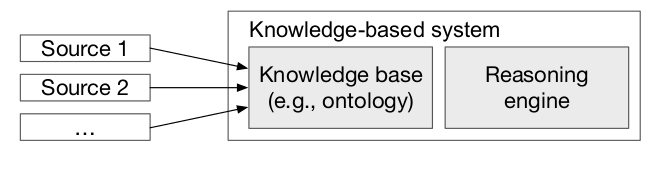
\includegraphics[scale=0.5]{KG}
    \caption{Struttura di un KG}
    \label{fig:KG}
\end{figure}


\section{Virtual Knowledge Graph}
\label{sec:vkg_description}
Specializzazione rispetto a un normale KG

Struttura di un vkg: ontology, mapping, schema

\section{Il Virtual Knowledge Graph system Ontop}
\label{sec:vkg_ontop}
VKG system open source che segue gli standard W3C 

\subsection{Intermediate Query language}
Ontop era inizialmente basato su Datalog poi passato ad un proprio linguaggio interno (Intermediate Query)

IQ: rappresentazione usata per tradurre le query degli utenti in SPARQL nelle query SQL dei mapping

\subsection{Esempi di utilizzo}
Esempi di utilizzo di Ontop in ambienti aziendali e accademici


